\documentclass[a4paper,12pt]{article}
  \usepackage{graphicx}
  \usepackage{indentfirst}
  \title{Deep Learning for Identifying Metastatic Breast Cancer}
  \author{Dayong Wang \emph{et al.}}
  \date{2016}

\begin{document}
\maketitle

\section{Contribution}

We present a deep learning-based approach for the identification of cancer metastases from whole slide images of breast sentinel lymph nodes.

Our system won both competitions at the Camelyon Grand Challenge 2016, with performance approaching human level accuracy. Combining the predictions of our deep learning system with a pathologist’s interpretations produced a significant reduction in the pathologist’s error rate.

\section{Method}

\subsection{Image Pre-processing}

To identify tissue within the WSI and exclude background white space, we first transfer the original image from the RGB color space to the HSV color space, then the optimal threshold values in each channel are computed using the \textbf{Otsu algorithm}, and the final mask images are generated by combining the masks from H and S channels.

\subsection{Cancer Metastasis Detection Framework}

Our cancer metastasis detection framework consists of a \textbf{patch-based classification} stage and a \textbf{heatmap-based post-processing} stage, as depicted in Fig. 1.

\begin{figure}[ht]
	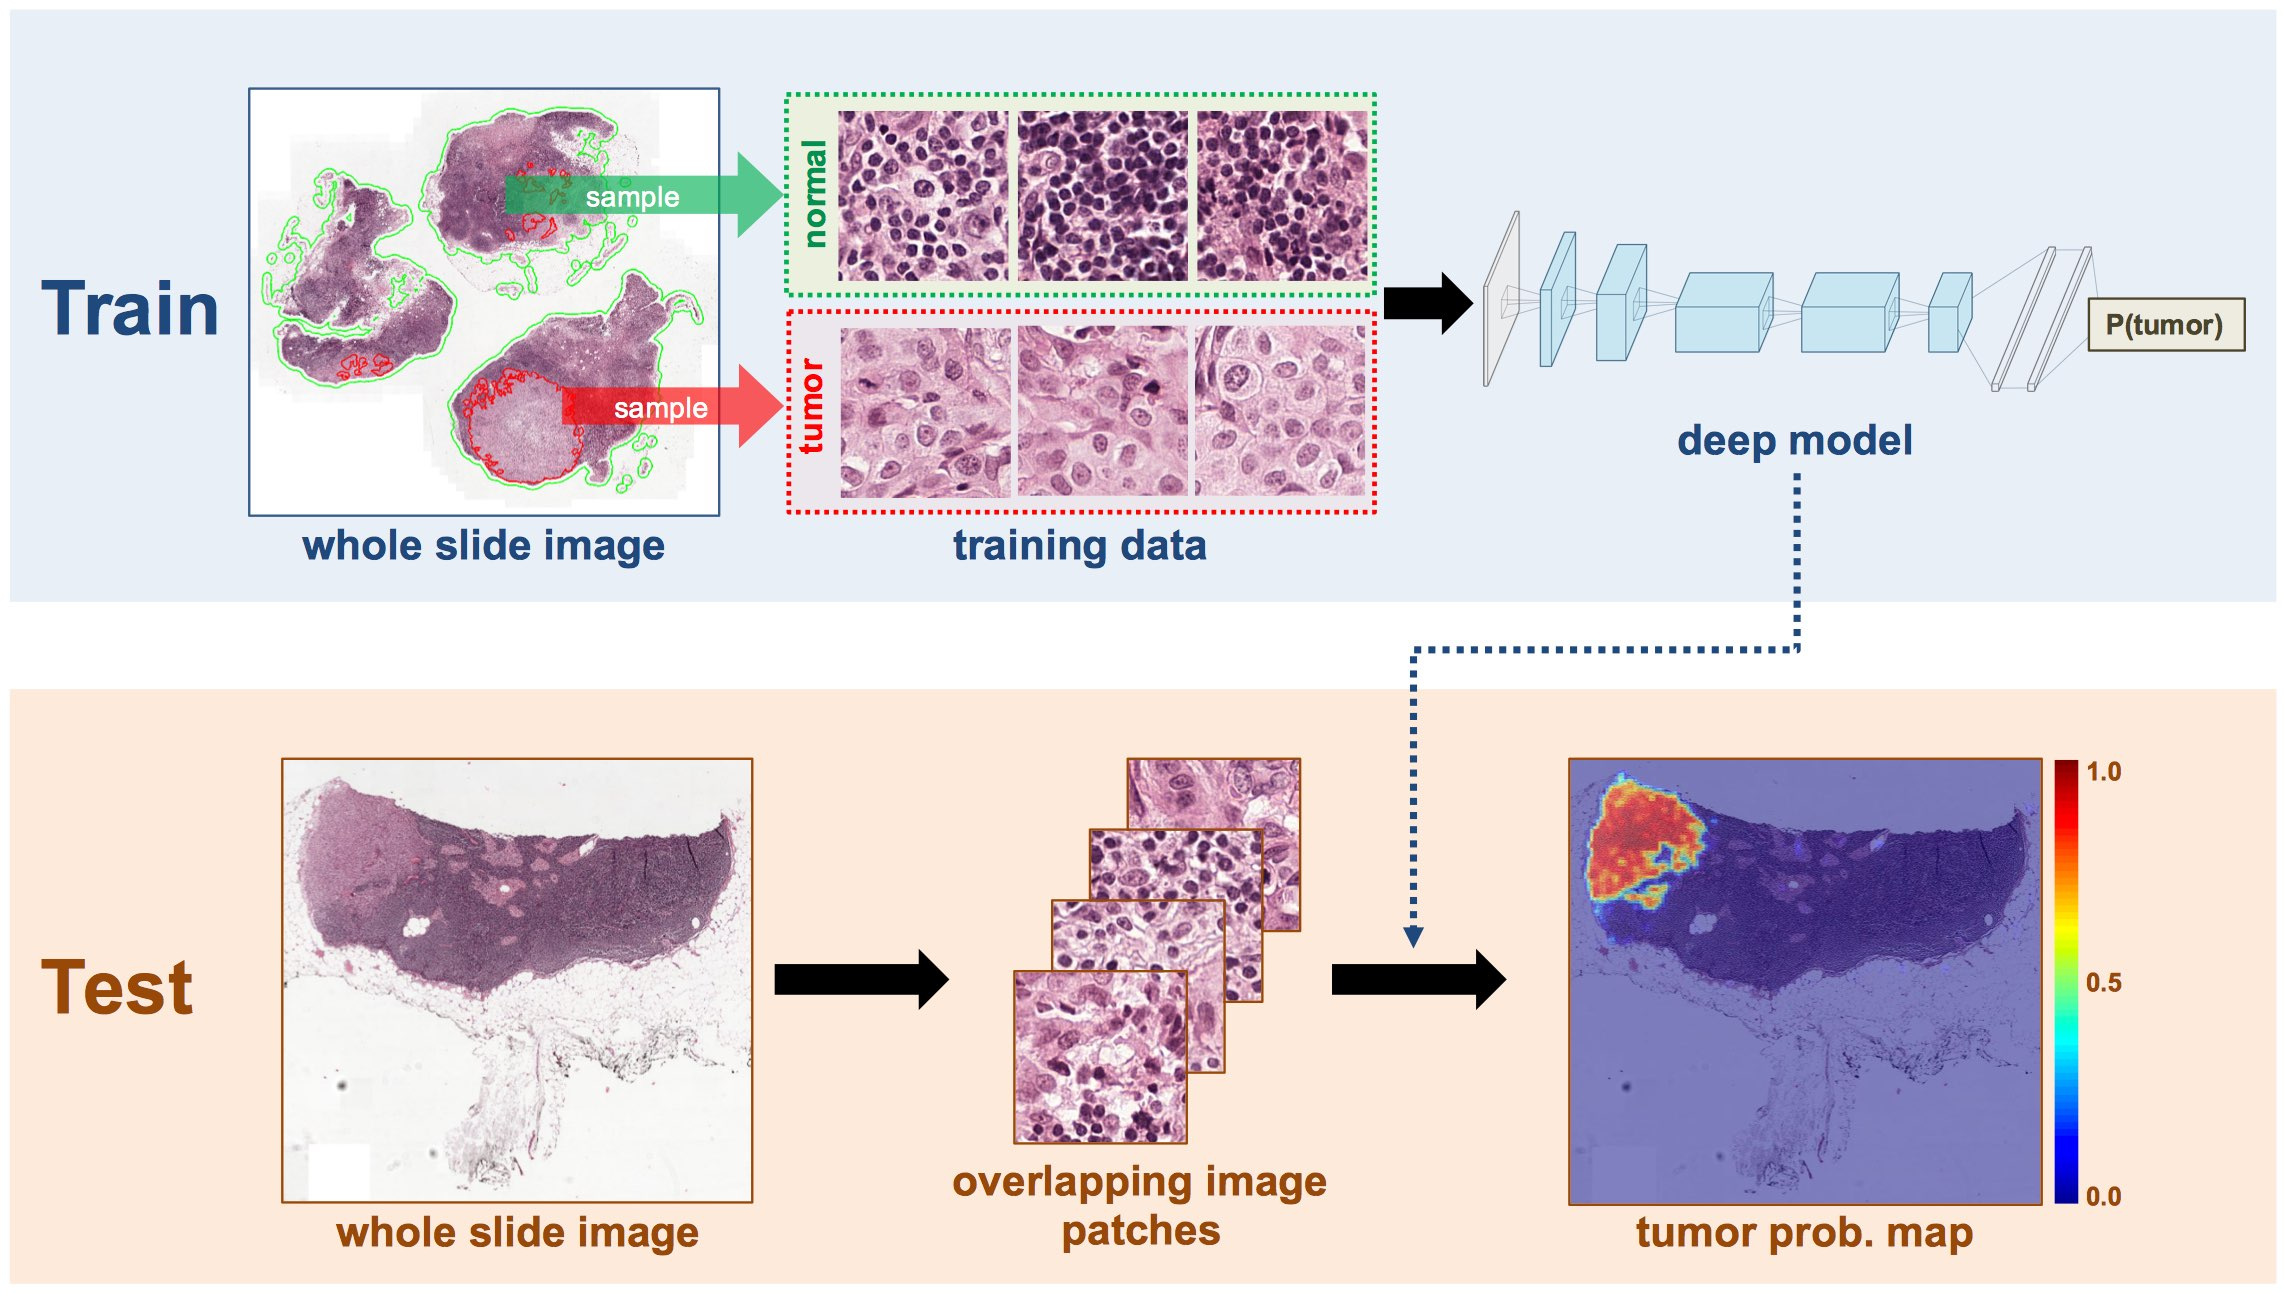
\includegraphics[width=\columnwidth]{img/metastasis-framework.jpg}
	\caption{The framework of cancer metastases detection.}
\end{figure}

\subsection{Patch-based Classification Stage}

During training, this stage uses as input 256x256 pixel patches from positive and negative regions of the WSIs and trains a classification model to discriminate between the positive and negative patches.

In our framework, we adopt GoogLeNet as our deep network structure since it is generally faster and more stable than VGG16.

In our experiments, we evaluated a range of magnification levels, including $40 \times$, $20 \times$ and $10 \times$, and we obtained the best performance with \textbf{$40 \times$ magnification}.

We noted that a significant proportion of errors were due to false positive classification from histologic mimics of cancer. To improve model performance on these regions, we extract additional training examples from these difficult negative regions and retrain the model with a training set enriched for these \textbf{hard negative} patches.

\subsection{Post-processing of tumor heatmaps}

On generated heatmaps, each pixel contains a value between 0 and 1, indicating the probability that the pixel contains tumor. We now perform post-processing to compute slide-based and lesion-based scores for each heatmap.

\subsubsection{Slide-based Classification}

Given a heatmap, we compute 28 geometrical and morphological features over tumor probability heatmaps (including the percentage of tumor region over the whole tissue region, the area ratio between tumor region and the minimum surrounding convex region, the average prediction values, and the longest axis of the tumor region) to build a \textbf{random forest classifier} to discriminate the WSIs with metastases from the negative WSIs.

\subsubsection{Lesion-based Detection}

\begin{enumerate}
	\setlength\itemsep{0em}
	\item Train a deep model (D-I) using our initial training dataset described above.
	\item Train a second deep model (D-II) with a training set that is enriched for tumor-adjacent negative regions, which produces fewer false positives than D-I but has reduced sensitivity.
	\item Threshold the heatmap produced from D-I at 0.90, which creates a binary heatmap.
	\item Identify connected components within the tumor binary mask, and use the central point as the tumor location for each connected component.
	\item Take the average of the tumor probability predictions generated by D-I and D-II across each connected component to estimate the probability at each of these $(x, y)$ locations.
\end{enumerate}

\section{Results}

\begin{itemize}
	\setlength\itemsep{0em}
	\item \emph{Slide-based Evaluation}: AUC (area under the ROC curve) score 0.9250.
	\item \emph{Lesion-based Evaluation}: FROC (free-response receiver operating characteristic) score 0.7051.
\end{itemize}

\subsection{Combining Deep Learning System with a Human Pathologist}

For the slide-based classification task,the human pathologist achieved an AUC of 0.9664, reflecting a 3.4 per-cent error rate. When the predictions of our deep learning system were combined with the predictions of the human pathologist, the AUC was raised to 0.9948 reflecting a drop in the error rate to 0.52 percent.

\section{Discussion}

The errors made by our deep learning system were \emph{not} strongly correlated with the errors made by a human pathologist.

Thus, integrating deep learning-based approaches into the work-flow of the diagnostic pathologist could drive improvements in the reproducibility, accuracy and clinical value of pathological diagnoses.

\end{document}
